\section{Results}\label{sec:results}
\hl{Note to scrutineers: all results shown are for pure-damping control.
I am still generating the results for reactive control and will include them when they are ready.}
\subsection{Design Space Exploration}
The OAT design sweep, shown in \figureautorefname~\ref{fig:experiments}, immediately draws attention to the float diameter $D_f$, shown with a red dashed line, as the variable with the strongest effect on the objectives.
A slight reduction in the diameter from its nominal value causes the cost to decrease close to linearly but the LCOE to skyrocket due to a substantial reduction in power generation.
Meanwhile, slightly increasing the diameter causes the power production to grow significantly but increases loads, leading to fatigue failure of the damping plate.
This is shown as blank on the diagram to indicate infeasibility.
A larger $\sim30\%$ diameter increase restores feasibility of the damping plate and achieves a roughly 15\textcent/kWh reduction in LCOE, representing the best design of the OAT sweep.
The results also point to the possibility of an even lower LCOE design with float diameter perhaps $\sim20\%$ larger than nominal, if the damping plate can be made feasible by increasing $t_d$ or $h_{1,stiff,d}$ without a major cost penalty. 

\begin{figure}
\centering
\includegraphics[width=\linewidth]{\matlabFilepath{15}}
\caption{Design of experiments}\label{fig:experiments}
\end{figure}

Besides $D_f$, the other design variable displaying a non-monotonic relationship with $LCOE$ is the force limit $F_{max}$, with an optimal at around half the nominal force limit.
Together, these insights inform the selection of the starting design for optimization, $\vec{x}_o$.
The OAT sweep also does not reveal any multimodality in the objectives, a promising sign that only a limited number of multi-starts may be necessary, although objective multimodality could still exist in other parts of the design space.
Finally, the OAT design sweep shows the highly constrained nature of the problem, with large regions of the design space infeasible.
In particular, the feasible region $1.3<D_f/D_{f,nom}<2.1$ is an ``island'' in the feasible design space, separated from the other feasible points at $D_f/D_{f,nom}<1 $ by the damping plate fatigue constraint.
Thus even without objective multimodality, multimodality exists in the Lagrangian (objective plus weighted active constraints), indicating the need for a multi-start optimization procedure as planned.

%\hl{Maybe add a 2D sweep of $D_f$ and $T_{f,2}$ if I have time}

\subsection{Single Objective Optimization}
\label{sec:results-single}
\subsubsection{Optimal Design}
\
In the single objective optimizations, $LCOE$ and $CAPEX$ are minimized and average power $P_{elec,avg}$ is maximized.
The SQP algorithm is executed starting with an initial condition corresponding to the nominal RM3 configuration.
For this $\vec{x_0}$, the optimizations all converge successfully.
Optimal designs ($\vec{x}^*=\text{argmin } J(\vec{x})$) are shown visually in \figureautorefname~\ref{fig:overlaid-geometry} and numerically in \tablename~\ref{tab:opt-dv-values}.
Also shown for comparison is the nominal design and a balanced design.
The latter is a $CAPEX$ minimization run with an additional constraint that the average power must exceed \powerBalanced~kW, a number chosen based on the shape of the multi-objective pareto front that will be presented in section \ref{sec:results-multi} with the intent of obtaining a cost reduction at the expense of a small power reduction compared to the minimum LCOE design.
This would be preferred whenever design-dependent capital expenditures carry greater importance than modeled here, such as with shorter-duration projects, higher discount rates, lower operational cost, and lower design-independent capital cost.

\begin{figure}
\centering
\includegraphics[width=\linewidth]{\matlabFilepath{23}}
\caption{Geometries overlaid}
\label{fig:overlaid-geometry}
\end{figure}

\begin{table}
\input{  \tableFilepath{19} }
\caption{Optimal design variables}\label{tab:opt-dv-values}
\end{table}

The optimal designs are generally larger than the nominal design.
The minimum LCOE design is larger in all bulk dimensions, with a particularly large increase in the float diameter, nearly doubling from 20~m to \DfoptMinLCOE~m.
It has a similarly sized PTO with a slightly lower maximum force rating and slightly higher maximum power rating.
Each of the other optimization objectives tested maintain this lower maximum force, while the maximum power rating is less consistent, with optimal values both higher and lower than the nominal.

In all optima, the three structural thicknesses are significantly decreased, and the float stiffener height decreases moderately.
This indicates that the optimized floats experience lower hydrodynamic forces and can reduce their structural material accordingly.
In the minimum LCOE design, the lower damping plate thickness occurs in favor of larger damping plate stiffeners, mimicking the observed paradigm in the aerospace industry where sheet metal skin just a few millimeters thick and substantial stiffeners are favored over thicker plate stock.
In fact, in several scenarios, structural thickness variables converge to their lower bounds.
The activity of these bound constraints, which represent priority 2 requirements in the language of section~\ref{sec:requirements}, indicates that the structures model is at the edge of its validity for describing thin-skinned stiffened shells.
Specifically, the assumption that the deflection field resembles that of a plate rather than that of a beam (see \appendixname~\ref{sec:appendix-structures}) is called into question.
Future expansion of the structures model to remove this assumption could allow the optimization to yield even more efficient structural designs.
Meanwhile in the minimum cost design, the damping plate stiffeners decrease in size. 

%\hl{discuss the difference between material reductions driven by structural load decrease versus structural efficiency increase, and how to tell the difference and which is happening here.}

Upon comparing the above-water geometric profiles of the nominal design with that of the pareto-optimal designs, a consistent trend emerges: the long support tubes of the nominal design have been replaced by a taller float and shorter support tubes.
This likely occurs because the slamming constraint $g_{NL,23}-g_{NL,239}$ encourages higher draft $T_{f,2}$, and the float height $h_f$ correspondingly grows since the submersion fraction of the float, $T_{f,2}/h_f$, is held constant as a parameter.

\subsubsection{Optimal Performance Outputs}
Next, analysis on the performance of the optimal designs yields insights into why these designs emerge as optimal.
The hydrodynamic coefficients and power distributions of each single-objective optimal design, along with the nominal design, are compared in Figures \ref{fig:overlaid-hydro} and \ref{fig:overlaid-power-dist} respectively.
The numerical results are shown in \tablename~\ref{tab:opt-output}.

\begin{figure}
\centering
\includegraphics[width=\linewidth]{\matlabFilepath{24}}
\caption{Hydrodynamic coefficients overlaid}
\label{fig:overlaid-hydro}
\end{figure}
\begin{figure}
\centering
\includegraphics[width=\linewidth]{\matlabFilepath{25}}
\caption{Cumulative distribution function of average power over time}
\label{fig:overlaid-power-dist}
\end{figure}
%\hl{describe which applications are best suited to which design. Maybe do min-LCOE, more expensive but could be min LCOE under some different economic scenario, cheaper and 10kW PBE, and cheaper and 1kW PBE.}

%This design is recommended for applications that are highly sensitive to the cost of energy and where energy storage is relatively cheap and abundant or there are dispatchable loads. This encompasses utility-scale installations and integrated generation-storage concepts such as a WEC coupled with offshore hydrogen production or pumped hydro. 

%On the opposite end of the spectrum, a second design is the least variable design, with an LCOE of \$1.00/kWh and merely 58\% power variation. This design is recommended for applications where the cost of energy is less critical, and storage is extremely limited. Powering the Blue Economy (PBE) applications such as aquaculture farms and AUV charging likely meet these criteria. 

%Finally, we recommend the balanced design for intermediate applications, where energy storage is available but not abundant, and cost is important but not the bottom line. An example is a grid-connected application for island communities. This balanced design has an LCOE of \$0.18/kWh and a power coefficient of variation equal to 100\%. 
%Further insight on the power profiles of these recommended designs compared to the baseline can be uncovered through probability distribution plots, shown in Figure \ref{fig:power-dist}. The minimum variation design is seen to be tuned to produce most of its power from moderate sea states only ($\sim$60-300 kW), whereas the minimum LCOE design has a much broader spectrum, collecting significant power both below 10~kW and above 1~MW. The balanced design falls in the middle. %As expected, the minimum LCOE design operates at high powers the most, spending 50\% of the time above 500~kW, compared to 40\% and 10\% for the balanced and minimum variation designs respectively. Also as expected, the minimum variation design spends a large amount of time ($\approx$40\%) at low powers below 50~kW. Interestingly, the minimum-LCOE design actually spends more time at low powers than the balanced design. In future work, the power distributions could be optimized more explicitly, incorporating information other than the coefficient of variation as an objective based on grid-level analysis.

\begin{table}
\input{  \tableFilepath{20} }
\caption{Optimal outputs}\label{tab:opt-output}
\end{table}

The minimum LCOE design achieves an annual average electrical power of \powerAvgAtMinLCOE~kW with a structural material mass of \structMassAtMinLCOE~kg and requires a generator rated for \powerMaxAtMinLCOE~kW and \forceMaxAtMinLCOE~kN peak.
This makes its estimated capital cost equal to \capexAtMinLCOE~\$M, of which \capexDesignAtMinLCOE~\$M comes from components modeled here as design-dependent (structural material and PTO size), and its estimated LCOE equal to \minLCOE~\$/kWh under the economic assumptions described in section~\ref{sec:econ}.
This is a \pctImproveLCOEMinLCOE~LCOE improvement over the nominal design's \nominalLCOE~\$/kWh, created through a simultaneous \pctImproveDesignCostMinLCOE~reduction in design-dependent cost and an \pctImprovePowerMinLCOE~increase in average power.
This LCOE is still far from that achievable with other renewables, with onshore wind and solar currently at 0.03-0.05~\$/kWh, fixed-bottom offshore wind currently at 0.11-0.14~\$/kWh, and floating offshore wind projected to be 0.11-0.25~\$/kWh in 2030 \cite{national_renewable_energy_laboratory_2024_2024}.

The CAPEX minimization shows that it is possible to reduce the design-dependent cost by an additional \pctImproveDesignCostMinCapex~at the cost of a \pctWorsePowerMinCapex~hit in average power, while the power maximization shows the option of increasing power by an additional \pctImprovePowerMaxPower~at the expense of a \pctWorseDesignCostMaxPower~increase in design-dependent cost compared to the minimum LCOE design.

Finally, \figureautorefname~\ref{fig:power-matrix-opt} shows a multiplicative breakdown of the power matrix for the minimum LCOE design.
The maximum capture width refers to the maximum capture width of any shape oscillating in heave based on the far-field radiation pattern.
The radiation efficiency describes the ratio of the maximum lossless power for the given shape to the maximum radiation-limited power, where the former refers to the power obtained with the design's hydrodynamic coefficents, no drag, and an unsaturated controller of the type specified by the parameters (either damping or reactive).
The drag efficiency describes the impact of turning on drag to the maximum lossless power, and increases with wave height as expected.
The $F_{max}$ factor describes the impact of the force limit, which departs from unity only at high wave heights and the resonant frequency of around 10 seconds.
Finally, the electrical efficiency describes the impact of the generator efficiency and the power limit.
Multiplying by the hours per year in each sea state expressed as a percentage yields the annual energy production.
\begin{figure}
    \centering
    \includegraphics[width=1\linewidth]{\matlabFilepath{PowerMultOpt}}
    \caption{Power matrix multiplicative breakdown for minimum LCOE design}
    \label{fig:power-matrix-opt}
\end{figure}

\subsubsection{Post-Optimality Derivatives}
Section~\ref{sec:single-obj-process} introduced the Lagrange multipliers $\vec{\lambda}=-dJ^*/d\vec{g}$ to quantify the activity and influence of constraints at the optimal point.
Values of the nonzero Lagrange multipliers $\vec{\lambda}$ are reported in \figureautorefname~\ref{fig:lagrange-multiplier}, signifying the increase in objective $J$ for a given increase in active constraint $\vec{g}$.

\begin{figure}
\centering
\includegraphics[width=\linewidth]{\matlabFilepath{15.5}}
\caption{Lagrange multipliers for LCOE-minimization}\label{fig:lagrange-multiplier}
\end{figure}

There are six active constraints at the optimum: one structural thickness lower bound, three structural factors of safety, and two amplitude constraints.
Interestingly, while the maximum (storm) DLC limits the float and damping plate, it is the operational (fatigue) DLC that drives the column sizing.
The amplitude constraints and the factor of safety on the damping plate in the storm DLC have the highest values of $\lambda$, indicating that these limits drive the optimal cost.
This motivates a potential future search for creative designs to obviate or mitigate the effect of these constraints, such as underwater submersion as an alternative storm survival technique, and investigating the tradeoff of using bump stops, active control, or other solutions to limit the device amplitude without increasing the dimensions.
Meanwhile, the activity of the float thickness lower bound and its larger value of $\lambda$ than the float FOS constraint indicates that the float structural model is inadequate in this regime and should be extended to better incorporate local buckling effects that would come to dominate for very thin-skinned designs.

Additional outputs of the optimization are the gradient of the objective, $\vec{\nabla} J=\partial J/\partial \vec{x}$, and the Hessian of the Lagrangian, $\textbf{H} = \partial^2 (J+\sum_i g_i)/\partial \vec{x}^2$.
They are shown in \appendixautorefname~\ref{sec:appendix-supplemental-results} since they are not particularly informative by themselves, especially since the gradient is expected to be zero at the optimum for all design variables not involved in an active constraint.
The utility of the gradient and Hessian are in their ability to calculate other local sensitivity measures, such as the impact of a design variable or parameter that is perturbed from its optimal value. Local parameter sensitivity analysis occurs in \sectionautorefname~\ref{sec:sensitivities-local}, and design variable perturbation is examined here.

\figureautorefname~\ref{fig:delta-J} shows the relative change in objective for a 10\% perturbation of each design variable from its optimal value, $\Delta J/J$, calculated using equation \eqref{eq:delta-J} and compared against the ``ground truth'' value from simulation re-evaluation.

\begin{equation}\label{eq:delta-J}
    \Delta J \approx \vec{\nabla} J^T \Delta \vec{x}% + \frac{1}{2} \Delta \vec{x}^T H \Delta \vec{x}
\end{equation}

\begin{figure}
\centering
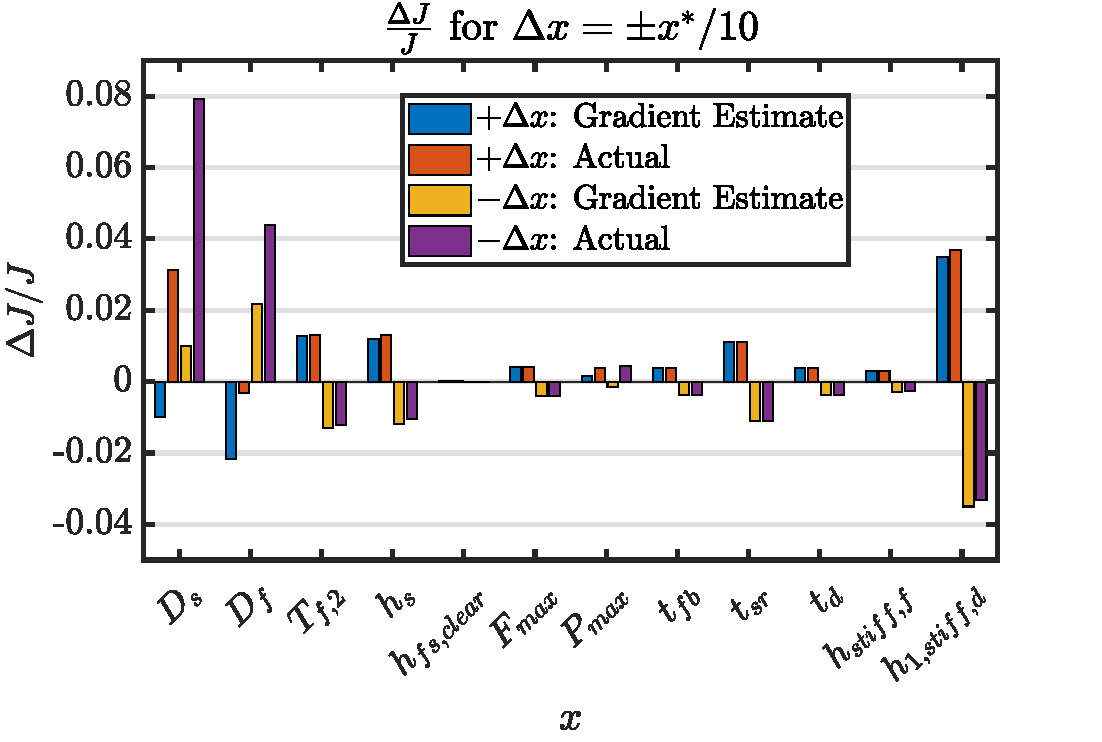
\includegraphics[width=\linewidth]{figs/delta_x.pdf}
\caption{Change in objective for perturbation of design variables from the minimum LCOE design}\label{fig:delta-J}
\end{figure}

The design variables with the highest sensitivities are $D_s$, $D_f$,and $h_{stiff,f}$, with a 10\% decrease in the diameters and 10\% increase in the stiffener height leading to a 7.9\%, 4.4\%, and 3.7\% increase in LCOE respectively.
The remaining design variables have a notably low sensitivity, meaning that they can be perturbed from their optimal value by 10\% in either direction without affecting the objective by more than 1-2\% (although they may affect constraints).
Finally, the gradient estimates are generally accurate, with the exception of the diameters $D_s$ and $D_f$ and the peak power $P_{max}$.
For these variables, nonlinearity or curvature exists in the objective function, indicating a tradeoff in the objective that would produce an optimum even without any active constraints.
For the case of LCOE minimization, this is expected because increasing the diameters and power rating both increase the power production while simultaneously increasing the capital cost.
More accurate estimates of the perturbed LCOE can be obtained by using the Hessian of the objective to account for curvature, but this would need to be obtained via manual finite differences because the solver only returns the Hessian of the Lagrangian.

\subsubsection{Multi-Start}
Separately, because non-convex optimization can get stuck in a local minimum, 1000 random initial guesses are tested, although 974 are linear infeasible and discarded.
Of the 26 linear feasible starting points, none converge while meeting the Karush-Kuhn-Tucker (KKT) conditions for first-order optimality.
For the LCOE-minimization, 17 optimizations converge due to small steps in the design while 9 fail to converge, and for the design cost minimization, that split is reversed, 9 and 17.
Of the optimizations that converge, 5 and 4 from the LCOE and design cost minimization respectively converge to the same minimum, referred to here as the global minimum since it is the lowest objective obtained across all starting points, although global optimality is never guaranteed.
On the other hand, more points (12 and 5 respectively) converge to a less optimal local minimum.
Of the optimizations that fail to converge, only one arrives at the same global minimum in each case.
\figureautorefname~\ref{fig:multistart-tree} shows this behavior on a probability tree.
Overall, around one fifth of the optimizations converge to the presumed global minimum.
Therefore, for a 95\% chance of obtaining the global optimum, a multi-start with at least $\textrm{ceil}\left(\frac{\ln(1-0.95)}{\ln(1-0.2)}\right)=\numMultistartRequired$ linear feasible starting points is required.
%\hl{XX}\% converged to the same point as the initial optimization did and none converged to a more optimal solution. While this does not guarantee a global optimum, the insensitivity to initial guess increases our confidence in the optimization results. 
\hl{Note to scrutineers: due to the high amount of linear infeasibility, I am going to try this again but generate points that are linear feasible from the start.}

\begin{figure}
\centering
\includegraphics[width=\linewidth]{\matlabFilepath{15.6_3}}
\caption{Probability tree for convergence of multi-start}\label{fig:multistart-tree}
\end{figure}

It is also worth investigating which characteristics of the starting point contribute to the outcome of the optimization. 
\figureautorefname~\ref{fig:multistart-bar} shows a bar chart of the convergence behavior as a function of the starting point for each design variable.
It shows that the float draft $T_{f,2}$ and float bottom plate thickness $t_{f,b}$ usually converge to the same optimal $\vec{x}^*$ value regardless of the starting point $\vec{x_0}$, but the other design variables are very sensitive to starting point.
This sheds light on the convexity of the search space, indicating that the float draft and bottom plate thickness are close to unimodal, while the other design variables are highly multimodal.

\begin{figure}
\centering
\includegraphics[width=\linewidth]{example-image-a}
\caption{Bar chart showing impact of starting point on convergence behavior}\label{fig:multistart-bar}
\end{figure}

Future studies can use this knowledge to potentially reduce the total number of function evaluations required to achieve the global optimum.
For example, to reduce the number of iterations within each optimization, the multistart procedure could use deterministic starting points for the float draft and bottom plate thickness, since sampling is necessary only for the multimodal design variables.
Meanwhile, the number of optimizations could be reduced by sampling multimodal variables from a non-uniform distribution to capture both multiple local minima.
More complete multistart results are shown in \appendixautorefname~\ref{sec:appendix-supplemental-results}.

% \begin{table}
% \begin{tabular}{c|c|c}
%    Objective & Cost & Power \\ \hline
%    Converged to any solution & XX & XX \\
%    Converged to same optimum & XX & XX \\
%    Converged to better optimum & 0 & 0 \\
% \end{tabular}
% \caption{Sensitivity to starting point}
% \end{table}

\subsection{Single Objective Sensitivity Analysis}\label{sec:sensitivities}
\subsubsection{Local Sensitivity to Parameters}\label{sec:sensitivities-local}
It is useful to start with local parameter sensitivity results.
The present section focuses on interpreting the results of the most accurate local sensitivty method: perturbing each parameter a small amount from its nominal value and repeating the optimization, while \appendixautorefname~\ref{sec:appendix-sensitivties} compares the accuracy and computation time of multiple computation methods.
The re-optimization accounts for nonlinearities and is thus more accurate but requires significantly more computation time to obtain than local sensitivities obtained with post-optimality derivatives.

\figureautorefname~\ref{fig:param-sens-J-star-tornado}, \ref{fig:param-sens-x-star-tornado}, and \ref{fig:param-sens-x-star-tornado-2} show Tornado charts for the parameters with highest normalized sensitivities for the objective and design respectively.
Results are normalized such that a value of 1 means that a given percent increase in the parameter from its nominal value causes the same percent increase in  $J^*$ or $x^*$.
\begin{figure}
    \centering
    \includegraphics[width=1\linewidth]{\matlabFilepath{16}}
    \caption{Tornado chart showing highest objective sensitivities}
    \label{fig:param-sens-J-star-tornado}
\end{figure}

Analyzing the left side of \figureautorefname~\ref{fig:param-sens-J-star-tornado}, the value of the minimum LCOE is highly sensitive to the operational wave characteristics, with normalized sensitivities of $-1.4$.
This means that a 1\% increase in wave height or period leads to a 1.4\% decrease in LCOE due to increased power production.
Meanwhile, the LCOE is also sensitive to array availability and transmission efficiency (normalized sensitivity $-1.0$) and PTO efficiency (normalized sensitivity $-0.8$).
The 1:1 correspondence for array efficiency is expected since it directly multiplies the annual energy production, as is the slightly lower value for PTO efficiency since it multiplies energy only in the sea states which are not at the power limit.
Another high sensitivity is the fixed charge rate ($FCR$), at a value of $+0.84$.
While modeled as constant in MDOcean, the $FCR$ itself scales positively with the interest rate (normalized sensitivity $+0.21$) and negatively with device lifetime (normalized sensitivity $-0.45$).
This puts the normalized sensitivity of LCOE to interest rate and lifetime at $+0.18$ and $-0.38$ respectively.

Moving to the right side of \figureautorefname~\ref{fig:param-sens-J-star-tornado}, overall the sensitivities are higher: the minimum LCOE has 5 parameters with normalized sensitivity magnitude above 0.5, whereas the minimum design cost has sixteen such parameters.
The minimum design cost is most sensitive (normalized value $+2.1$) to the nondimensional damping plate stiffener height $h_{stiff,d}/h_{1,stiff,d}$, indicating that future optimizations should consider adding this as a design variable.
Other high sensitivities including $D_d/D_s$ ($+1.7$), $D_{d,tu}$ ($-1.6$), $D_{d,min}$ ($-1.1$), and $w_{stiff,d}/h_{1,stiff,d}$ ($-1.0$) also relate to the damping plate geometry and no float or spar geometric parameters have high sensitivity, indicating that the damping plate design drives the minimum achievable cost.
This begs the question whether it is worth having the damping plate at all, or if WECs with a low power, low cost design objective would do better to remove the need for a damping plate by fixing the spar to the sea floor, if the water is sufficiently shallow to do so.
This comparison is worth quantifying in future optimization studies. 

Meanwhile, the price of power $\$/W$ also has a high normalized sensitivity ($-2.1$), though notably the price of force $\$/N$ has too low a sensitivity to appear on the chart.
Site parameters ($h$, $-1.8$; $H_s$, $-1.6$; $T_{struct}$, $+1.4$; and $H_{s,struct}$, $+1.1$) also have high sensitivities, though interestingly the sign of the sensitivity for $T_{struct}$ has changed compared to the minimum LCOE point, such that a larger structural period decreases the minimum LCOE but increases the minimum design cost.
Based on the $N_{WEC}$ sensitivity, adding an additional WEC to the 100-WEC array will decrease the minimum per-WEC design cost by $1.1\%$ due to the economies of scale built into the economic model, an effect not observed in the LCOE minimization.
Unintuitively, the sensitivity to the material yield strength is positive ($+1.0$), such that a stronger material results in a more expensive design.
This is because with several structural thicknesses at their lower bound, the structural cost cannot be significantly reduced, and instead the added strength is leveraged by moving to a more expensive design with larger bulk dimensions and higher loads. %\hl{(This still doesn't make sense, the larger bulk design would only be chosen over the baseline design if it made the cost lower, since power is the held the same as a constraint for the min-cost optimization).}
Finally, the minimum design cost is sensitive to material density and cost (both $+0.6$).
This indicates the potential desirability of a lighter, cheaper material for the low power WEC.
The two sensitivities are expected to be equal due to the mass-based material cost model.

\begin{landscape}
\begin{figure}
    \centering
    \includegraphics[width=1\linewidth]{\matlabFilepath{17}}

    \caption{Tornado chart showing highest design variable sensitivities at minimum LCOE}
    \label{fig:param-sens-x-star-tornado}
\fillandplacepagenumber
\end{figure}
\end{landscape}
\begin{landscape}
\begin{figure}
    \centering
    \includegraphics[width=1\linewidth]{\matlabFilepath{18}}
    \caption{Tornado chart showing highest design variable sensitivities at minimum design cost}
    \label{fig:param-sens-x-star-tornado-2}
\fillandplacepagenumber
\end{figure}

 \end{landscape}
%Figure~\ref{fig:constraint-sens} gives the estimated parameter change threshold required to make inactive constraints active and active constraints inactive. Values are again normalized, where here a value of 1 means that a parameter would need to double (increase by 100\%) before the constraint activity changes.

Meanwhile, \figureautorefname~\ref{fig:param-sens-x-star-tornado} depicts sensitivity of optimal design variables to parameters, $\frac{d\vec{x}^*}{d\vec{p}}$. 
Unlike the objective sensitivities, which describe the effect of parameter changes on WEC viability, the design variable sensitivities describe the effect of parameter changes on the optimal design. 
For parameters representing uncontrollable external inputs, such as many site parameters, high values indicate a need for certainty of the parameter value early in the design cycle to ensure that the ultimate design is appropriate for the real parameter values.
For parameters representing controllable design choices that were held fixed rather than optimized for the sake of simplicity, such as many geometric parameters, high values indicate that future studies should include the value as a design variable instead of a parameter.

The design variable values which minimize LCOE are most sensitive to site (black) and geometric (red) parameters, with a subset of structural design variables ($t_{sr}$, $h_{stiff,f}$, and $h_{1,stiff,d}$) also being sensitive to structural (yellow) parameters.
In \figureautorefname~\ref{fig:param-sens-x-star-tornado-2}, the design variables which minimize design cost are sensitive to these three parameter categories plus economic parameters.
Dynamic parameters (blue), including the float and spar drag coefficients and PTO efficiency, do not significantly affect the optimal design in either case.
The low sensitivity to the drag coefficients in particular is notable because it means that it is likely not necessary to expend additional model development effort to capture the variation in drag coefficient with hull shape, wave frequency, material surface roughness, or other quantities.
It is also apparent that some of the structural thicknesses ($t_{fb}$ and $t_d$ in both optimizations, and $t_{sr}$ in the design cost minimization) are insensitive to all parameters because the optimal value is consistently at the lower bound.
This reinforces the aforementioned need for future enhancements to the structures model to better capture local buckling behavior for thin-skinned stiffened shells.

Looking at geometric parameters more specifically to assess if any should become design variables, we observe that $D_d/D_s$ strongly (normalized value above 0.5) affects the optimal values of four design variables ($D_s$, $t_sr$, $h_s$, and $h_{stiff,f}$), indicating that $D_d$ should be a design variable in future optimizations to ensure the coupling is adequately captured.
The parameter driving the float draft slant angle, $T_{f,1}/T_{f,2}$, has a high effect on the overall draft $T_{f,2}$, indicating that $T_{f,1}$ should also be a design variable.
The parameter driving the spar slenderness, $T_s/D_s$, significantly affects the spar height and float spar clearance $h_s$ and $h_{fs,clear}$, indicating that $T_s$ should be added as a design variable in addition to $h_s$.
Finally, the amount of clearance between the float and spar, $D_{f,in}/D_s$, has a large effect on  $h_{stiff,f}$.
This might suggest the addition of $D_{f,in}$ as a design variable, but a more significant gap between the float and spar would change the hydrodynamics in a way that is not modeled due to moonpool resonance effects, making this addition less straightforward than others. 
%\hl{Any other params that could have been design variables, show that the sensitivity is hopefully low.}
In summary, the parameters that should be added as design variables in future optimizations are $D_d$, $T_{f,1}$, $T_s$, and possibly $D_{f,in}$.

%Highly sensitive parameters include \hl{XXX}.
%Insensitive parameters include \hl{XXX.
%Describe which are sensitive to J vs x vs constraint activity.
%Maybe also show dJ/dx and that's important because you need that DV exact or not without affecting your bottom line.}
%\hl{Is it possible to use these sensitivities to demonstrate coupling, and predict the effect of holding some DVs constant?) - during re scrutineering} 

%For these highly sensitive parameters, it is worthwhile to perform a global sensitivity analysis to observe any nonlinearity. Figure~\ref{fig:param-sens-global} and \ref{fig:x-opt-sens-global} demonstrate the new optimal objective and optimal design variable values respectively under the re-optimization-based OAT global parameter sensitivity process described in section~\ref{sec:single-obj-process}.
% \begin{figure}\label{fig:param-sens-global}
% \includegraphics[width=\linewidth]{example-image-a}
% \caption{Global OAT parameter sensitivity analysis to optimal objective $J^*$}
% \end{figure}
% \begin{figure}\label{fig:x-opt-sens-global}
% \includegraphics{example-image-a}
% \caption{Global OAT parameter sensitivity analysis to optimal design $x^*$}
% \end{figure}

%The global sensitivity analysis indicates that \hl{list parameters} have strongly nonlinear sensitivities over the range of interest. During re-scrutineering. \hl{Sentence interpreting any params that aren't location based}. 

\subsubsection{Global Sensitivity to Deployment Location}
The high sensitivity to wave conditions warrants further analysis.
An additional global sensitivity analysis is conducted by reoptimizing for several discrete deployment locations.
This captures any interactions between the simultaneous changes to wave height, wave period, water depth, and storm sea state which previous local sensitivity analysis cannot capture due to its OAT nature.
Additionally, it shows the effect of different bandwidth seas, or the tendency for energy to be concentrated in one frequency or spread out across the spectrum, which is not captured in the previous results.
This will reveal not only which locations are most favorable for WEC deployment through the resulting LCOE, but also whether the optimal WEC design is robust to location through the resulting optimal design variables.
The effect of wave conditions on design is especially important considering that global deployability is a core requirement for WEC viability \cite{bull_systems_2017} and the ability to use a single WEC design across different wave conditions facilitates economies of scale and design convergence.

Wave resource data for four U.S. locations (Humboldt Bay, California; Pac-Wave North, Oregon; Pac-Wave South, Oregon; and Wave Energy Test Site, Hawaii) is obtained from the NREL SAM repository \cite{janzou_sam_2022}, which sources its data from a 2015 report by Sandia National Lab \cite{dallman_characterization_2015}.
All economic assumptions are held fixed for consistency, which neglects the effect of location-specific bathymetry on foundation cost and distance from shore on installation, operations, and maintenance costs.
The optimal design variables and LCOE corresponding to each of the four locations are shown in Table~\ref{tab:location}.

\begin{table}\label{tab:location}\setlength\arraycolsep{1pt}
\begin{tabular}{>{\centering\arraybackslash}p{0.22\linewidth}>{\centering\arraybackslash}p{0.08\linewidth}>{\centering\arraybackslash}p{0.17\linewidth}>{\centering\arraybackslash}p{0.17\linewidth}>{\centering\arraybackslash}p{0.17\linewidth}>{\centering\arraybackslash}p{0.18\linewidth}}
&& \multicolumn{4}{c}{Location}\\  \cline{3-6} 
& Symbol & Humboldt, CA & PacWave North, OR & PacWave South, OR & Wave Energy Test Site, HI\\ 
\hline 
Most frequent wave & - & $H_s = 1.25$m, $T_e=7.5$s & $H_s = 1.25$m, $T_e=8.5$s & $H_s = 1.75$m, $T_e=8.5$s & $H_s = 1.75$m, $T_e=6.5$s \\ 
Incident energy flux (kW/m) & $J$ & $32.2 $ & $37 $ & $40.7 $ & $14.3 $ \\ 
Half-power bandwidth (rad/s) & $BW$ & $390 \cdot 10^{-3}$ & $250 \cdot 10^{-3}$ & $240 \cdot 10^{-3}$ & $370 \cdot 10^{-3}$ \\ 
%Storm sea states (m, s) & $H_{s,storm},T_{e,storm}$ &  &  &  &  \\ 
Water depth (m) & $h$ & $45 $ & $50 $ & $65 $ & $55 $ \\ 
Opt. spar diameter & $D_s^*$ & $6 $ & $6 $ & $6 $ & $6 $ \\ 
Opt. float diameter & $D_f^*$ & $27.9 $ & $25.1 $ & $26.9 $ & $37.3 $ \\ 
Opt. float draft & $T_{f,2}^*$ & $990 \cdot 10^{-3}$ & $990 \cdot 10^{-3}$ & $990 \cdot 10^{-3}$ & $4.31 $ \\ 
Opt. spar height & $h_s^*$ & $38.4 $ & $38.6 $ & $39.7 $ & $39.5 $ \\ 
Opt. float-spar clearance height & $h_{fs,clear}^*$ & $3.9 $ & $3.93 $ & $3.99 $ & $1.8 $ \\ 
Opt. maximum force & $F_{max}^*$ & $2.44 $ & $3.36 $ & $6.61 $ & $2.98 $ \\ 
Opt. maximum power & $P_{max}^*$ & $286 $ & $286 $ & $286 $ & $288 $ \\ 
Opt. float bottom thickness & $t_{fb}^*$ & $13.4 $ & $13.7 $ & $14.2 $ & $1.27 $ \\ 
Opt. spar radial thickness & $t_{sr}^*$ & $25 $ & $25.1 $ & $25.4 $ & $7.21 $ \\ 
Opt. damping plate thickness & $t_d^*$ & $25 $ & $25.2 $ & $25.4 $ & $1.31 $ \\ 
Opt. float stiffener height & $h_{stiff,f}^*$ & $170 \cdot 10^{-3}$ & $196 \cdot 10^{-3}$ & $249 \cdot 10^{-3}$ & $261 \cdot 10^{-3}$ \\ 
Opt. damping plate stiffener height & $h_{1,stiff,d}^*$ & $389 \cdot 10^{-3}$ & $423 \cdot 10^{-3}$ & $585 \cdot 10^{-3}$ & $956 \cdot 10^{-3}$ \\ 
Opt. levelized cost of energy (\$/kWh) & $LCOE^*$ & $605 \cdot 10^{-3}$ & $605 \cdot 10^{-3}$ & $539 \cdot 10^{-3}$ & $513 \cdot 10^{-3}$ \\ 
\end{tabular}
\caption{Results for Re-Optimization in Four Distinct Locations}
\end{table}

All optimized LCOE values are less expensive than the RM3 baseline.
The WEC located in Pac-Wave South, OR results in the lowest LCOE, \$\LCOEPacWaveNorth/kWh, which makes sense because the incident wave energy flux is highest there.
The WEC located in WETS, HI has the highest LCOE, \$\LCOEHawaii/kWh, aligning with its low incident energy.
The values of the optimal design are similar for the California and Oregon locations, but quite different for Hawaii, with the latter having a \HawaiiDesignCharacteristics.
This is surprising: using the simple scaling argument $\omega_n = \sqrt{\frac{k}{m}}=\sqrt{\frac{\rho g A}{\rho A T_f C_m}}\sim T_f^{-\frac{1}{2}}$ a WEC's uncontrolled natural frequency scales with its draft to the $\frac{-1}{2}$ power, so a smaller draft would be expected in sites with higher-frequency waves like Hawaii.
One hypothesis for this reversal is that Hawaii's lower incident energy and thus lower wave excitation force requires a higher oscillation amplitude to achieve comparable energy production, which in turn necessitates a higher draft to avoid slamming.
\hl{(I'm not sure if this is the true explanation, need to inspect intermediate results to confirm.)}
This result demonstrates the importance of using a full coupled model to optimize WEC design, as the simple scaling heuristic produces an inaccurate conclusion.
\hl{(Note: I may replace one of the PacWaves with North Carolina so I have a result from the East coast.
I would also like to include the results of holding design constant, ie with each output row having another row below it showing the ratio from using} $x^*_{California}$ at that location).

%\subsubsection{Price Global Sensitivity}
%We also perform a global sensitivity analysis for price parameters $p_\tau$, $p_P$, $p_M$, and $p_0$ from equation~\eqref{eq:LCOE-scale}. For $p_0$, if the design-independent (unmodeled) cost goes to zero, \hl{(and maybe change 80\% efficiency into 100\%)}, that's essentially the best LCOE that a WEC of these technical assumptions (steel point absorber with given operational conditions) can get. We can think of the rest as a cost gap \hl{(explain)}. Meanwhile, the global sensitivity analysis for $p_\tau$ gives preliminary insight into the multi-objective problem, recovering a portion of the pareto front between the four variables that influence $LCOE$: $\tau$, $P_{pk,elec}$, $V_{struct}$, and $P_{avg,elec}$. This shows \hl{XXX conclusion}, to be clarified further in the multi-objective optimization.

\subsubsection{Global Sensitivity to Modeling Assumptions}
\label{sec:sensitivity-model-assumptions}
In addition to continuous parameters, the simulation depends on discrete options that dictate model behavior.
These settings include the control scheme (damping or reactive), the presence of generator force saturation, the presence of drag, and the number of dynamic degrees of freedom (float heave motion only or float and spar heave motion).

\paragraph{Control Scheme}
\hl{This analysis is left for during scrutineering.}

\paragraph{Force Saturation}
First examining the optimal LCOE design presented in \sectionautorefname~\ref{sec:results-single}, the lowest force saturation power factor across all sea states in \figureautorefname~\ref{fig:power-matrix-opt} is $\frac{P_{sat}}{P_{unsat}}=\lowestFmaxFactorMinLCOE$, with a corresponding force limit of $\frac{F_{max}}{F_{unsat}}=\lowestFsatMinLCOE$~in that sea state. 
%This corresponds almost exactly with the relationship expected in the purely resistive Thevenin impedance case in \cite{mccabe_force-limited_2024}:
%\begin{equation}
%   \frac{ P_{sat}}{P_{unsat}}=1-\left(\frac{F_{max}}{F_{unsat}}-1\right)^2
%\end{equation}
% see notebook p46 5/16/25
% fixme: what about the factor of 4/pi in the force ratio? Then the quadratic equation wouldn't apply, it would be more complicated (alpha non zero case) which casts doubt on my conclusion that alpha=0 emerges as optimal. Would need to compute alpha directly I think? I also think that the assumption of damping control means my Im(Gamma)=0 assumption in the notebook is false. Also Psat/Punsat is the the same as Psat/Pmax. So leaving this sentence out.
Considering all sea states, the optimal force-saturated design sacrifices only \powerLossForceSatMinLCOE~Watts of average power (around \pctPowerLossForceSatMinLCOE) and reduces its PTO cost by \pctPTOSavingsForceSatMinLCOE, leading to an LCOE reduction of \pctImproveLCOEForceSatMinLCOE~compared to the same design with no force saturation, although the unsaturated design violates structural constraints due to the higher force.
If the optimization is instead re-run to ensure constraint satisfaction while not allowing force saturation, the result has a \pctPowerLossForceSatOptMinLCOE~power gain, \pctPTOSavingsForceSatOptMinLCOE~higher PTO cost, \pctStructSavingsForceSatOptMinLCOE~higher structural cost, and \pctImproveLCOEForceSatOptMinLCOE~higher LCOE compared to the optimization with saturation.

\paragraph{Drag}
As section~\ref{sec:sensitivities-local} alludes to, the low sensitivity to drag coefficient suggests that modeling the drag nonlinearity is perhaps not essential.
This is surprising, because without drag the resonant amplitude is significantly higher, which should affect the results due to the active slamming constraint.
One reason for this discrepancy is that the drag sensitivity was local only, and a re-optimization at $C_d=0$ would likely yield different results.
\hl{Performing this re-optimization is left for during scrutineering.}

\paragraph{Degrees of Freedom}
\hl{This analysis is left for during scrutineering.}

\clearpage
\subsection{Multi-Objective Optimization}\label{sec:results-multi}
In the multi-objective optimization, the design-dependent capital cost $C_{design}$ and the average electrical power $P_{avg,elec}$ are optimized simultaneously to show the trade-off between the two quantities.
As described in section~\ref{sec:multi-obj-process}, the multi-objective analysis gives important insights for cases where the LCOE may not apply or is uncertain due to variation in cost variables modeled as constant, including $OPEX$, $FCR$, and $p_0$.
A pareto front is shown in Figure \ref{fig:pareto}, with the utopia point marked with a green star, simulated designs marked with squares, and the actual performance of the nominal design as reported in \cite{RM3} marked with a diamond.
All designs on the Pareto front have a significantly lower cost than the nominal RM3 design, with a range of powers both smaller and larger than the nominal.
Figure~\ref{fig:pareto-lcoe} provides a zoomed-in version with superimposed contours of constant $LCOE$ for reference.
The minimum LCOE design occurs at the point of tangency between the pareto front and the LCOE contours and very nearly coincides with the maximum power design. %\hl{analyze more: how are the max power and min LCOE designs different? talk about the multiple apparent points of tangency (ie at 50 cents/kWh) and whether those are local minimums in LCOE.}
\begin{figure}
    \centering
    \includegraphics[width=.8\linewidth]{\matlabFilepath{19}}
    \caption{Pareto Front}
    \label{fig:pareto}
\end{figure}
\begin{figure}
\centering
\includegraphics[width=.8\linewidth]{\matlabFilepath{20}}
\caption{Pareto front with different LCOE contours overlaid }
\label{fig:pareto-lcoe}
\end{figure}

There exists a cusp in the pareto front at the point where the average electrical power is around \powerWhereCusp~kW.
As a result of this cusp, the bulk of the pareto front (extending from the least-cost design at \powerAvgAtMinCapex~kW to around \powerWhereNonconvexEnds~kW) is non-convex.
This region would have been missed with a convex multi-objective optimization procedure that optimizes weighted sums of the objectives, affirming the necessity of the epsilon-constraint plus pattern search procedure used here.

Figure~\ref{fig:pareto} inlays geometry visualizations for a few designs highlighted in light blue.
One apparent trend is that the optimal spar draft and float diameter increase in size as one moves from left to right along the Pareto front.
This makes sense intuitively: to minimize material, the components will be as small as possible while satisfying constraints.
Larger dimensions incur higher costs and allow more power generation.

Similar trends are explored more quantitatively in Figure \ref{fig:design-heuristics}.
The graph provides extremely useful design heuristics for how to adapt WEC design to a given application, depending on the desired balance between cost and power output.
In the interest of showing consistent, easily interpretable trends even with random, non-uniform spacing of points, the x-axis shows the percent along the pareto front, calculated by scaling the angle of each pareto point from the nadir point, and the y-axis values are lightly smoothed with a low pass filter.
To facilitate comparison against the pareto front in Figure~\ref{fig:pareto} and visualize clusters, the individual pareto points are shown as black squares on the x-axis of Figure \ref{fig:design-heuristics}.
Structural design variables are green, powertrain ratings are blue, and bulk geometry dimensions are red. 
\begin{figure}
    \centering
    \includegraphics[width=1\linewidth]{\matlabFilepath{21}}
    \caption{Design and objective heuristics plot}
    \label{fig:design-heuristics}
\end{figure}

Analysis starts by examining the direction of the changes.
With increasing cost and increasing average power (from left to right in the figure), most design variables either monotonically increase ($P_{max}$, $D_s$, and $t_{s,r}$) or almost monotonically increase with one brief decline ($F_{max}$, $D_f$, $h_{1,stiff,d}$, and $h_s$).
Just two design variables are mainly decreasing: $T_{f,2}$ and $h_{fs,clear}$, both variables involved in the float amplitude constraints.
Two of the remaining three design variables ($t_d$ and $t_{f,b}$, structural thicknesses at their lower bound) stay constant across the pareto front with the exception of a few small upwards excursions in $t_d$ around 2\%, 23\%, and 60\% of the way through, while the final variable $h_{stiff,f}$ experiences several small oscillations. 

Analyzing the magnitude of changes, the powertrain ratings differ the most drastically across the pareto front, while geometric and structural variables require only moderate adjustments.
This begs the question: how much are the cost savings at lower powers driven by the smaller PTO cost compared to the smaller material cost?
If PTO cost dominates the savings, WEC companies selling devices at multiple power levels may want to maintain the same geometric and structural design across all products, changing only the PTO, which reduces design effort and facilitates economies of scale compared to changing all subsystems.
Using the cost values in the earlier Table~\ref{tab:opt-dv-values}, unfortunately only \pctCostSavingsFromPTO~of the cost savings come from the smaller PTO, indicating that for a lower power WEC under the previously stated price assumptions, the slightly smaller hydrodynamic design is actually much more important to pursue than the substantially smaller PTO.
Therefore, design reuse across varying power levels is unlikely.
This conclusion differs from preliminary work \cite{mccabe_multidisciplinary_2022} which wrongly examined only the change in the optimal design without taking into account the relative impact of PTO and device dimensions on cost.

Meanwhile, the bottom part of \figureautorefname~\ref{fig:design-heuristics} provides a similar insight on how values change across the pareto front for objectives instead of design variables. % change objectves to outputs - ie LCOE, CF, X_max, all the y* in single objective.
The power output is largely linear, while the design cost experiences a discrete change in slope at around 5\% and a gradual change beyond that.
The discrete slope change causes the aforementioned cusp in the pareto front, and the figure now elucidates that this corresponds to a change in PTO sizing strategy: from 0-5\% along, the cost-power tradeoff is achieved by adjusting the maximum power, whereas from 5-70\% along it is achieved by adjusting the maximum force while maintaining constant maximum power.
The gradual design cost slope change indicates diminishing returns (an increased marginal cost of additional power generation).

%An additional point of note on the Pareto front of Figure \ref{fig:pareto} is the LCOE and coefficient of variation of a typical solar array plotted for comparison (data from \cite{borettiSolar}). Even the cheapest WEC design is still almost an order of magnitude more expensive than solar, indicative of the immaturity of WEC technology and the need for further innovation and cost reduction. On the bright side, many of the designs achieve a lower coefficient of power variation than solar, indicating the potential for wave energy as a relatively steady grid-connected renewable. Finally, it is worth highlighting that the amount of power variation directly affects the required energy storage, so the local cost of storage affects the position along the Pareto front that is optimal for a given application.

%We can plot LCOE contours under different economic assumptions (sweep a couple FCRs, p0s, and opexes) and overlay this to the results already obtained in the global sensitivity analysis of FCR, p0, and opex but now plotted in multiobjective space.\hl{(Explain this better)}

Figure~\ref{fig:constraint-activity} shows which optimization constraints are active along the pareto front.
Three structural design variables ($t_d$, $h_{stiff,f}$, and $h_{1,stiff,d}$) hit their lower bound, while none hit their upper bound.
The only linear constraint active is the spar natural frequency constraint.
Since this constraint was marked as priority two (required for modeling accuracy given the assumptions), its activity is significant and will be discussed more in section~\ref{sec:discussion}.
Aside from the irrelevant maximum force constraint, which is always active by design, active nonlinear constraints include the float, column, and damping plate structural factors of safety, and the amplitude constraints preventing the float from rising above the spar, maintaining linear wave theory, and preventing slamming of the float.
\begin{figure}
    \centering
    \includegraphics[width=1\linewidth]{\matlabFilepath{22}}
    \caption{Constraint Activity}
    \label{fig:constraint-activity}
\end{figure}

%\hl{If there's room/time, consider a bonus pareto of LCOE vs CF.}

%\subsection{Multi-Objective Sensitivity Analysis}
%\hl{This section I don't have results for yet and can be cut if needed. Maybe show trace out the effect of parameter variation without reoptimizing in multiobjective space, and it shows you how far some param variations bring you from optimal, like the dJ/dp sensitivities before but now for everywhere on the pareto front, and visualized differently. Perhaps also do re-optimized pareto fronts for a parameter or two that was found to be highly influential in the single objective analysis. Also show the effect of keeping geometric DVs fixed and what the new pareto front and design heuristics curve would look like.}

\subsection{Optimization Runtime}
Figure \ref{fig:optim-runtimes} shows the runtime for each optimization and analysis routine, as run in parallel on the 14-core server described in section~\ref{sec:sim-runtime}. 
The optimization also runs without issue, albeit more slowly, on unspecialized machines such as a Windows 10 laptop computer with MATLAB R2022a.

\begin{figure}
\centering
\includegraphics[width=\linewidth]{\matlabFilepath{26}}
\caption{Bar chart of optimization and analysis runtimes}
\label{fig:optim-runtimes}
\end{figure}
%the standard GitHub Linux runner for public repositories, which has 4 CPUs and 16 GB RAM with Ubuntu 24.04 operating system.
Each single-objective optimization takes just \singleObjRuntime, converging in \singleObjIters~iterations and requiring \singleObjFcnEvals~function evaluations including both objective and gradient evaluation. 
Generating the pareto front takes \paretoRuntime, of which \paretoPctTimeSeeds~is spent generating seeds via epsilon-constraint and the remaining \paretoPctTimePatternSearch~on the pattern search. 
Gradient-based post-optimality sensitivities run rapidly in just \gradientSensRuntime, while sensitivities obtained via re-optimization take \reoptimSensRuntime.

\figurename~\ref{fig:pareto-epsilon-runtime-sweep} shows the effect of the number of epsilon-constraint seeds on the number of function evaluations and hypervolume. (\hl{Analysis is left for during scrutineering.})

\begin{figure}
\centering
\includegraphics[width=\linewidth]{example-image-a}
\caption{Effect of number of epsilon-constraint seeds on pareto front function evaluations and hypervolume}
\label{fig:pareto-epsilon-runtime-sweep}
\end{figure}
